\documentclass{article}
\usepackage{amsmath}
\usepackage{txfonts}
\usepackage{booktabs}
\usepackage{color}
\usepackage{bussproofs}
\usepackage{graphicx}
\usepackage{pifont}
\usepackage{qtree}
\usepackage{tikz}
\usepackage{amssymb}
\usetikzlibrary{automata,arrows,positioning,calc}
\usepackage{listings}
\usepackage{hyperref}
\newenvironment{scprooftree}[1]%
{\gdef\scalefactor{#1}\begin{center}\proofSkipAmount \leavevmode}%
{\scalebox{\scalefactor}{\DisplayProof}\proofSkipAmount \end{center} }

\begin{document}
\lstset{language=Java}
\author{Jappie Klooster}
\title{Agents and you, a brief summary}
\maketitle

\section{Introduction}
This will be an introduction to agents coming from someone who followed
` hbo informatica' as pre study.

In here I will write down the things I think are important.

\section{Modal logic}


\section{APL}
Medhi dastani taught about the agent programming langauge (APL).
\subsection{Agent data structure}
This represents the mental state of a agent. \\
\begin{tabular}{ll}
	Name & Does what \\ \toprule
	Beliefs & Information available to the agent \\
	Goals & Objectives that the agent wants to achieve \\
	Events & Obsevations of (environmental) changes \\
	Capabilities & Actions that the agent can perform \\
	Plans & Procedures to achieve objectives \\
	Reasoning rules & Reason about goal and plans \\
\end{tabular} \\

\noindent
The rules can be:

\begin{itemize}
	\item Planning rules (goal $\to$ plan)
	\item Procedural rules (events $\to$ plan)
	\item Plan repair rules (plan $\to$ plan)
\end{itemize}

\subsection{Processing mental states}

\begin{itemize}
	\item Generate plans for received events.
	\item Generate plans for goals.
	\item Process exceptions and handle failures.
	\item Repair plans.
	\item Select plans for execution.
	\item Execute plans.
\end{itemize}

\subsection{Operational semantics}
Operational semantics defines the computation steps a program
configuration may take. Operational semantics allows studying
of programming constructs in a rigorous manner. It facilitates proving
general properties about a language. It lies close to the implementation
of an interpreter. It facilitates model checking.

\subsubsection{Basic syntax}
The configuration $C$ evolves into configuration $C'$:

\[C \to C'\]

If premise $P$ holds transition $C \to C'$ can be derived:

\begin{prooftree}
	\AxiomC{$P$}
	\UnaryInfC{$C \to C'$}
\end{prooftree}

\subsection{Configuration}
configurations only mention things that change.
Multi-agent configuration where $A$ is an agent and $\chi$ is the
environment:

\[\langle \{A_1, \cdots, A_n\}, \chi\rangle \]

Individual agent configuration where $i$ is the agent number, $\sigma$ the
believes, $\gamma$ the goals, $\Pi$ the plans $\theta$ the assignments and
$\xi$ the events:

\[A_i = \langle i, \sigma_i, \gamma_i, \Pi_i, \theta_i, \xi_i \rangle \]

\subsection{Transitions}
The confiugrations described \emph{what} can change where transition
will describe \emph{how} they can change.

$\vDash$ Describes a first order entailment relation. As I understand
this means $A \vDash B$ there exsits a $B$ in $A$ which has an entailment
to $A$. So $A$ is a set of things and a $B$ like thing exists in $A$.
\subsubsection{Belief update}
Execution of a belief update action $\alpha$ modifies the belief and goal
bases. $Update$ is an update function that is specified by the believe
update actions and $\gamma'=\gamma - \{\psi \in \gamma | \sigma' \vDash \psi\}$.
Which basically says that $\gamma'$ is equal to $\gamma$ minus the update.

\begin{prooftree}
	\AxiomC{$Update(\sigma, \alpha\theta)=\sigma'$}
	\UnaryInfC{$\langle i, \sigma, \gamma, \{(\alpha,id)\}, \theta, 
		\xi\rangle \to 
	\langle \langle i, \sigma', \gamma', \{\}, \theta, \xi\rangle$}

\end{prooftree}

So on the left side of the arrow, the plan is to do a believeUpdate $\alpha$
on the right side this is done so its removed from the plans and the believes
\emph{and} goals are modified. The goals are modified to because if a believe
with the same name as a goal becomes true than the goal is removed. (this is
a design decision btw, its just how 2apl works).

\subsubsection{Adopta goal}
Execution of a goal adopt action adopta(g) adds the goal to the beginning of
the goal base. If the goal $g$ trough assignment $\theta$ does not already
exists in goalbase.

\begin{prooftree}
	\AxiomC{$\sigma \nvDash g\theta$}
	\UnaryInfC{$\langle 
		i, \sigma, [\gamma_1, \cdots, y_n], \{(adopta(g),id)\}, \theta, \xi, 
	\rangle \to \langle 
		i, \sigma, [g\theta,\gamma_1, \cdots, y_n], \{\}, \theta, \xi, 
	\rangle$}
\end{prooftree}

So the agent comes accross a adopta method in the plan base $\Pi$, if
the associated believe of the goal is not true then you can start adding
it.
\subsubsection{Applying planning goal rules}
The structure of a PG-rule in 2apl is as follows:

\[\kappa <- \beta | \pi \]

Where $\kappa$ is the name of the plan.
$\beta$ is the condition that is applied before
executing the plan (basically a big if around the plan). $\pi$ is
the body of the plan, a set of instructions.

\begin{prooftree}
	\AxiomC{$\gamma \vDash \kappa \tau_1 \quad \& \quad
	\sigma \vDash \beta \tau_1 \tau_2$}
	\UnaryInfC{$\langle
		i, \sigma, \gamma, \Pi, \theta, \xi
	\rangle \to \langle
	i, \sigma, \gamma, \Pi \cup \{ \pi \tau_1 \tau_2 \}, \theta, \xi
	\rangle$}
\end{prooftree}

The transition can be executed if $\kappa$ is an active goal (this valuation
is stored in $\tau_1$ \emph{and} $\beta$ is true according to the believe 
base (this eveluation is stored in $\tau_2$). If all these things are true
then $\pi$ is added to the plan base $\Pi$ \emph{but} it will only be executed
if $\tau_1$ and $\tau_2$ return true.
\subsection{Exam}
some notes I gathered for possible exam questions:

What happens if $\gamma = pos(2,3)$ and $\sigma = pos(4,5)$, resolve with
state transitions.

\section{Markov}
Computerised decision makers must deal with an uncertain world.

\subsection{Expectation}
Excpectation is the average value you excpect to happen. For example if you
throw a dice the average value you should get is 3.5. Because:

\[1 * 1/6 + 2 * 1/6 + 3 * 1/6 + 4 * 1/6 + 5 * 1/6 + 6 * 1/6 = 3.5\]

You multiple all possible values time the chance of them happening and then
calculate the sum of them. Formally it is written like this:

\[ E[X]=Def \sum_{all x} xP\{X=x\} \]

So you can fill it in like:
\[E[X]= 1 * P\{X=1\} + \cdots + 6 *P\{X=6\}\]
\[E[X]= 1 * 1/6 + \cdots + 6 *1/6 = 3.5\]

\subsubsection{Properties of expectation}

\begin{itemize}
	\item $E[c] = c$
	\item $E[X+Y] = E[X] + E[Y]$
	\item $E[cX] = cE[X]$
	\item $E[XY] = E[X]E[Y]$ if and only if $X$ and $Y$ are independent.
	\item $E[X] \le E[Y]$, if $X \le Y$ almost surely.
\end{itemize}

\paragraph{Law of the onconcious statistician}
You have to prove this, its \emph{not} a property:

\[E[g(X)]=\sum_{all x} g(x)P{X=x}\]

where $g$ is any real-valued function. (It returns a value that is part
of the real set of numbers).

\subsection{Conditional expectation}
The expectation of $X | Y = y$ is called the \emph{conditional expectation}
of $X$ given $Y$, and is denoted by:

\[E[X|Y=y]\]

$E[X|Y=y]$ Is a number that depends on $y \in Y$. So you only get an
expectation $X$ if you have an y that satisfies the condition.
This yields a random variable $E[X|Y]$. Because of this it has all the
properties of a random variable.

\subsubsection{Probability mass functions}
The standart notation for probability mass functions is:

\[p_x(x): D(X) \to [0,1]: x \mapsto P\{X=x\} \]
\[p_y(y): D(Y) \to [0,1]: y \mapsto P\{Y=y\} \]
\[p_{xy}(x,y): D(X) \times D(Y) \to [0,1]: (x,y) \mapsto P\{X=x,Y=y\} \]
\[p_{x|y}(x|y): D(X) \times D(Y) \to [0,1]: (x,y) \mapsto P\{X=x|Y=y\} \]

For example:

\[ P\{X=x|Y=y\}=\frac{P\{X=x,Y=y\}}{P\{Y=y\}}\]

Is often written as:

\[P_{x|y}(x|y)=\frac{P_{xy}(x,y)}{P_y(y)}\]

\subsection{Total expectation}
The tower property, which is awesome:

Let $X$ and $Y$ be random variables then:

\[ E[E[X|Y]] = E[X] \]

The proof is in the slides.

\subsection{Markov to matrix}
A finite Markov process consisting of $n$ states can be represented by an 
$n\times n$ \emph{probablity transition matrix}.

Consider the following markov process:
\begin{center}
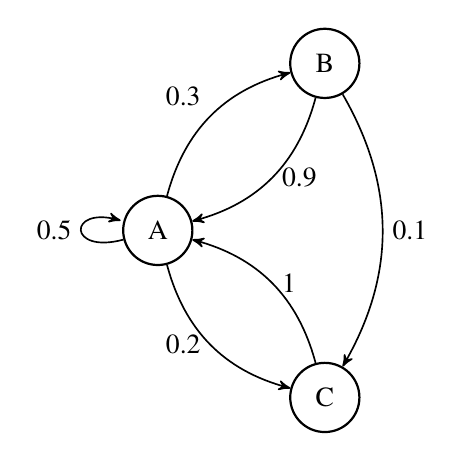
\begin{tikzpicture}[->, >=stealth', auto, semithick, node distance=3cm]
\tikzstyle{every state}=[fill=white,draw=black,thick,text=black,scale=1]
\node[state]    (A)                     {A};
\node[state]    (B)[above right of=A]   {B};
\node[state]    (C)[below right of=A]   {C};
\path
(A) edge[loop left]     node{0.5}         (A)
    edge[bend left]     node{0.3}     (B)
    edge[bend right, left]     node{0.2}      (C)
(B) edge[bend left,right]    node{0.9}      (A)
    edge[bend left,right]    node{0.1}      (C)
(C) edge[bend right, right]    node{1}      (A);
\end{tikzpicture}

The probability matrix belonging to this process looks like the following:

\[
\begin{matrix}
		& A		& B		& C \\
	A	& 0.5	& 0.3	& 0.2 \\
	B	& 0.9	& 0		& 0.1 \\
	C	& 1		& 0		& 0 \\
\end{matrix}
\]

\end{center}

Adding the $A,B,C$ is optional, but I find it gives more overview. The first
cell reads, the probobality of going from a to a.

\subsubsection{Stochastic}
A matrix where every row sums to1 is called a \emph{stochastic matrix}. Every
transition matrix is a \emph{stochastic matrix}.

\subsection{Sample path}
A \emph{sample path} of a markov chain is a specific specific realistion of
that chain.

\[ X_0,X_1,X_2,\dots\]

The $X_i$ are random variables.

\subsection{Markov process}
A \emph{Markov process} is a stochastic process $X_0, X_1, X_2, \dots$ such 
that:

\[ P\{ X_{n+1} X_n, X_{n-1}, \dots\}=P\{X_{n+1}|X_n\}\]
for $n \ge 0$

\subsubsection{Remarks}
If states are numbers, then often state space is denoted by $I$, with 
typical elements $i,j,k$.

A markov process is sometimes called a markov chain. These concepts are
equal.

If $S$ is countably infinite, then the probability transition matrix
can be represented as an ``open ended'' stochastic matrix.
\[
	P =
\begin{pmatrix}
	p_{1,1}	& p_{2,1}	& p_{3,1} & \cdots\\
	p_{1,2}	& p_{2,2}	& p_{3,2}	& \cdots\\
	p_{1,3}	& p_{2,3}	& p_{3,3}	& \cdots\\
	\vdots	& \vdots	& \vdots		& \ddots \\
\end{pmatrix}
\]
With markov proceci it is extremly important to beclear about the
\emph{cardinality of the state space} (finite, discrete, continues) and
the \emph{nature of time} (discrete, continuous)

A \emph{dead state} or a \emph{dead end} is a state that does not have
any outgoing arcs. An \emph{absorbing  state} is a state that has precisely
one outgoing arc with probability 1 to itself.

\subsection{Chapman-Kolmogorov equations}

\[P^{(n)}_{ij} = \sum_{all\mbox{\ }k} P^{(n_1)}_{ik} P^{(n_2)}_{kj} \]

It is convenient to list the $n$-step transition probabilities in a matrix.
\[
	P^{(n)} =
\begin{pmatrix}
	p^{(n)}_{1,1}	& \cdots	& p^{(n)}_{n,3} 	& \\
	\vdots	& \ddots	& \vdots	& \\
	p^{(n)}_{1,n}	& \cdots	& p^{(n)}_{n,n}	& \\
\end{pmatrix}
\]

In particiular $P^{(1)} = P$.

\subsubsection{Lemma}
Suppose $k+l=n$ Where $k,l\ge1$. Then $P^{(k)} \cdot P^{(l)} = P^{(n)}$

(I think this was proven)

$P^{(n)} = P^n$, this was definitivley proven. Not sure why you would
prove removing brackets, but whatever.

\subsection{Classes}
No this aren't default private structures (its a c++ reference).

Classes make dealing with large markov chains easier by grouping nodes
together. \emph{Open classes} allow the process to escape the class once
it enters a \emph{closed class} it will remain there forever.
A class is \emph{Transient} if a process can never reenter it, a
state is recurrent if it can. A process is multichain if there are
multiple recurrent classes, if there is just one reccurent class
its uni-chain.

A critical transition is a transition between classes.

A closed class doesn't have to be recurrent if there are infinite cases.
Otherwise a closed class is always recurrent.
An openclass is always transient.

\subsection{Markov reward}
A \emph{Markov reward process} is a markov process with rewards on
transitions. these rewards are real valued.

Markov rewards processes are also known as \emph{markov reward chain} or
\emph{valued Markov chains}.

example

\[
	P =
\begin{pmatrix}
	0.2	& 0.8 & 0 	& \\
	0.3	& 0	& 0.7	& \\
	0	& 0 & 1	& \\
\end{pmatrix}
\]
With reward matrix:
\[
	R =
\begin{pmatrix}
	1	& 2 & 0 	& \\
	0	& 0	& 3	& \\
	0	& 0 & 0	& \\
\end{pmatrix}
\]

\subsubsection{Total reward}

Let $\omega$ be a realisation of a Markov process:

\[\omega = s_0, s_1, \dots\]

where $s_0$ is a start state.
The rewards that accumulate are $r_1, r_2, \dots$:

\[ s_0 \xrightarrow[\mbox{reward } r_1]{} s_1 \xrightarrow[\mbox{reward } r_2]{} s_2\]

\paragraph{Definition}

$r_k | (s_0=1) : $ reward at kth step, given $s_0 = i$.
$R|(s_0=i),$ the \emph{total reward} : $(r_1 + r_2 \dots)|s_0=i,$
$V(i),$ the \emph{value} of state i : $E[R|s_0=i]$.

\subsection{The bellman equation}

\[V(i)=\sum_{all\mbox{\ }j} p_{ij}[r_{ij} + V(j)]\]

This system of linear equations enables us to compute state values in two
ways, by using algebra or by using iteration. Iteration you just wait until
convergence within a specified range. For this course iteration is enough.

\subsection{Utility pump}
A utility pump is a MRP in which at least one recurrent state possesses a
non-zero reward.
\subsubsection{Discount factor}
A \emph{dicsount factor} is a real number $0 \le \gamma < 1$. it represents
the probability to survive from one state to the next.

\paragraph{remarks} The discount factor is constant. The discount factor
does not impose a fixed cuttoff bound. It is a probablistic concept.

\subsubsection{Discounted reward}
Suppose a discount factor $0 \le \gamma < 1$. Then

\[V(i)=\sum_{all\mbox{\ }j} p_{ij}[r_{ij} + \gamma V(j)]\]

for every state $i$.

\paragraph{definition} A \emph{valuation} is a vector

\[v=Def
\begin{pmatrix}
	v(1) \\
	\vdots \\
	v(n)
\end{pmatrix}
\in \mathbb{R}^n
\]

\paragraph{definition} The \emph{expected immediate reward} at state $i$ is
the by $P_{ij}$ - probabilities weighted averaga of the $r_{ij}$ rewards:

\[C(i)=Def\sum_{all \mbox{\ }j} p_{ij} r_{ij} \]

The (vertical) vector of expected immediate rewards is denoted by $C$.

\paragraph{definition} The \emph{Bellman operator}:

\[B_p : \mathbb{R}^n \to \mathbb{R}^n : v \mapsto C + \gamma Pv \]
\subsection{Exam}
 For a given decision problem with a certain
discount factor.A pure policy sufices.
Do policy iteration, (a single iteration), do value iteration
(single iteration).

\end{document}
